\documentclass[12pt,a4paper,titlepage]{article}

\usepackage{titlesec} %spacing for sections
\usepackage[utf8]{inputenc}	% Unicode support
\usepackage[margin=0.5in]{geometry}
\usepackage[pdftex]{graphicx}% Picture handling
	\graphicspath{C:/Users/Stefano\ Dalla\ Longa/Desktop/RETTLOGBrandoLonga/doc/}
	\DeclareGraphicsExtensions{.pdf,.jpeg,.png}
\usepackage{epstopdf}
\usepackage{listings}		% Formatting and highlighting

\author{Stefano Dalla Longa\\pID 10535602 \and Nicolò Brandolese\\pID 10531144}
\date{}
\title{Prova Finale di Reti Logiche, AA 2019-2020}


\begin{document}
	%title page
	\begin{titlepage}
    \begin{center}
        \vspace*{3cm}
            
        \Huge
        \textbf{Prova Finale di Reti Logiche}
            
        \vspace{0.5cm}
        \LARGE
        AA. 2019/2020
            
        \vspace{1.5cm}
            
        \textbf{Stefano Dalla Longa, pID 10535602 \\ Nicolò Brandolese, pID 10531144}
        
        \vspace{1.2 cm}
        \Large
		Politecnico di Milano, scaglione prof. Fornaciari
            
        \vspace{0.8cm}
            
    \end{center}
\end{titlepage}

	\tableofcontents
	\clearpage	%using \newpage gives a wrong table of content enumeration
	\section{Introduzione}
   
		This is the first section.
      
		Lorem  ipsum  dolor  sit  amet,  consectetuer  adipiscing  
		elit.   Etiam  lobortisfacilisis sem.  Nullam nec mi et 
		neque pharetra sollicitudin.  Praesent imperdietmi nec ante. 
		Donec ullamcorper, felis non sodales...
       
	\section{Descrizione della macchina}
		L'implementazione si basa sulla scomposizione in tre sottoproblemi:
		\begin{enumerate}
			\item comunicazione con la RAM, intesa come l'insieme di operazioni di lettura e scrittura
			\item computazione per determinare l'appartenenza dell'indirizzo base ad una working zone
			\item gestione del flusso in base al risultato della computazione
		\end{enumerate}
		La scelta di risoluzione è stata la creazione di una macchina a stati finiti, in particolare una macchina di Mealy, basata su tre macroprocessi:
		\begin{itemize}
			\item \textit{\texttt{state\_register}}: ad ogni fronte di salita del clock propaga il valore del prossimo stato della macchina \textit{\texttt{next\_state}} al registro dello stato corrente \textit{\texttt{current\_state}}. Reagisce al segnale di \textit{\texttt{i\_reset}} eseguendo un reset sincrono, ovvero assegnando invece il valore di \textit{\texttt{START\_IDLE}} a \textit{\texttt{current\_state}} sul fronte di salita del clock.
			\item \textit{\texttt{speak\_with\_RAM}}: gestisce i valori dei segnali in input e output, ad eccezione di \textit{\texttt{o\_done}} il quale è gestito da \textit{\texttt{calc\_process}}.
			\item \textit{\texttt{calc\_process}}: esegue i calcoli per determinare se l'indirizzo base appartiene alla working zone considerata
		\end{itemize}
		Al quale si aggiungono due ulteriori processi destinati alla gestione degli elementi di memoria interni:
		\begin{itemize}
			\item \textit{\texttt{wz\_counter\_process}}: aggiorna sul fronte di discesa del clock il contatore \textit{\texttt{wz\_counter}} delle working zone già controllate tramite il segnale \textit{\texttt{count\_add\_sig}}. Permette di resettare il suo contenuto a zero in caso di reset o di segnale di start portato a zero. L'aggiornamento sul fronte di discesa anziché di salita del clock risolve diversi problemi di sincronia tra il contatore e i successivi stati, dal momento che il suo valore deve disponibile allo stato immediatamente successivo all'aggiornamento del suo contenuto.
			\item \textit{\texttt{FF\_saving}}: gestisce i flip-flop relativi a quattro segnali da memorizzare. Non è stato necessario fornirlo di segnale di reset.
		\end{itemize}
		
		Abbiamo scelto di separare \textit{\texttt{calc\_process}} e \textit{\texttt{speak\_with\_RAM}} per ragioni di leggibilità, dal momento che da un punto di vista teorico entrambi costituiscono una componente combinatoria della stessa macchina a stati finiti, e perciò sarebbe stato possibile accorparli nel medesimo processo. Dal momento però che VHDL proibisce di modificare lo stesso segnale da processi diversi, la gestione del flusso modificando il valore di \textit{\texttt{next\_state}} è affidata esclusivamente a \textit{\texttt{calc\_process}}.
		\newline
		\newline
		Il funzionamento della macchina a stati è schematizzato nella figura seguente; gli stati in blu sono tutti e i soli stati nei quali opera \textit{\texttt{speak\_with\_RAM}} e sono progettati per durare un ciclo di clock, gli stati in verde sono gli stati di calcolo e codifica da parte di \textit{\texttt{calc\_process}} anch'essi progettati per cambiare ad ogni ciclo di clock, mentre gli stati in rosso sono stati di idle gestiti da \textit{\texttt{calc\_process}}, progettati per bloccare il flusso di esecuzione ed eventualmente ricominciare la computazione in base al valore di \textit{\texttt{i\_start}}.

		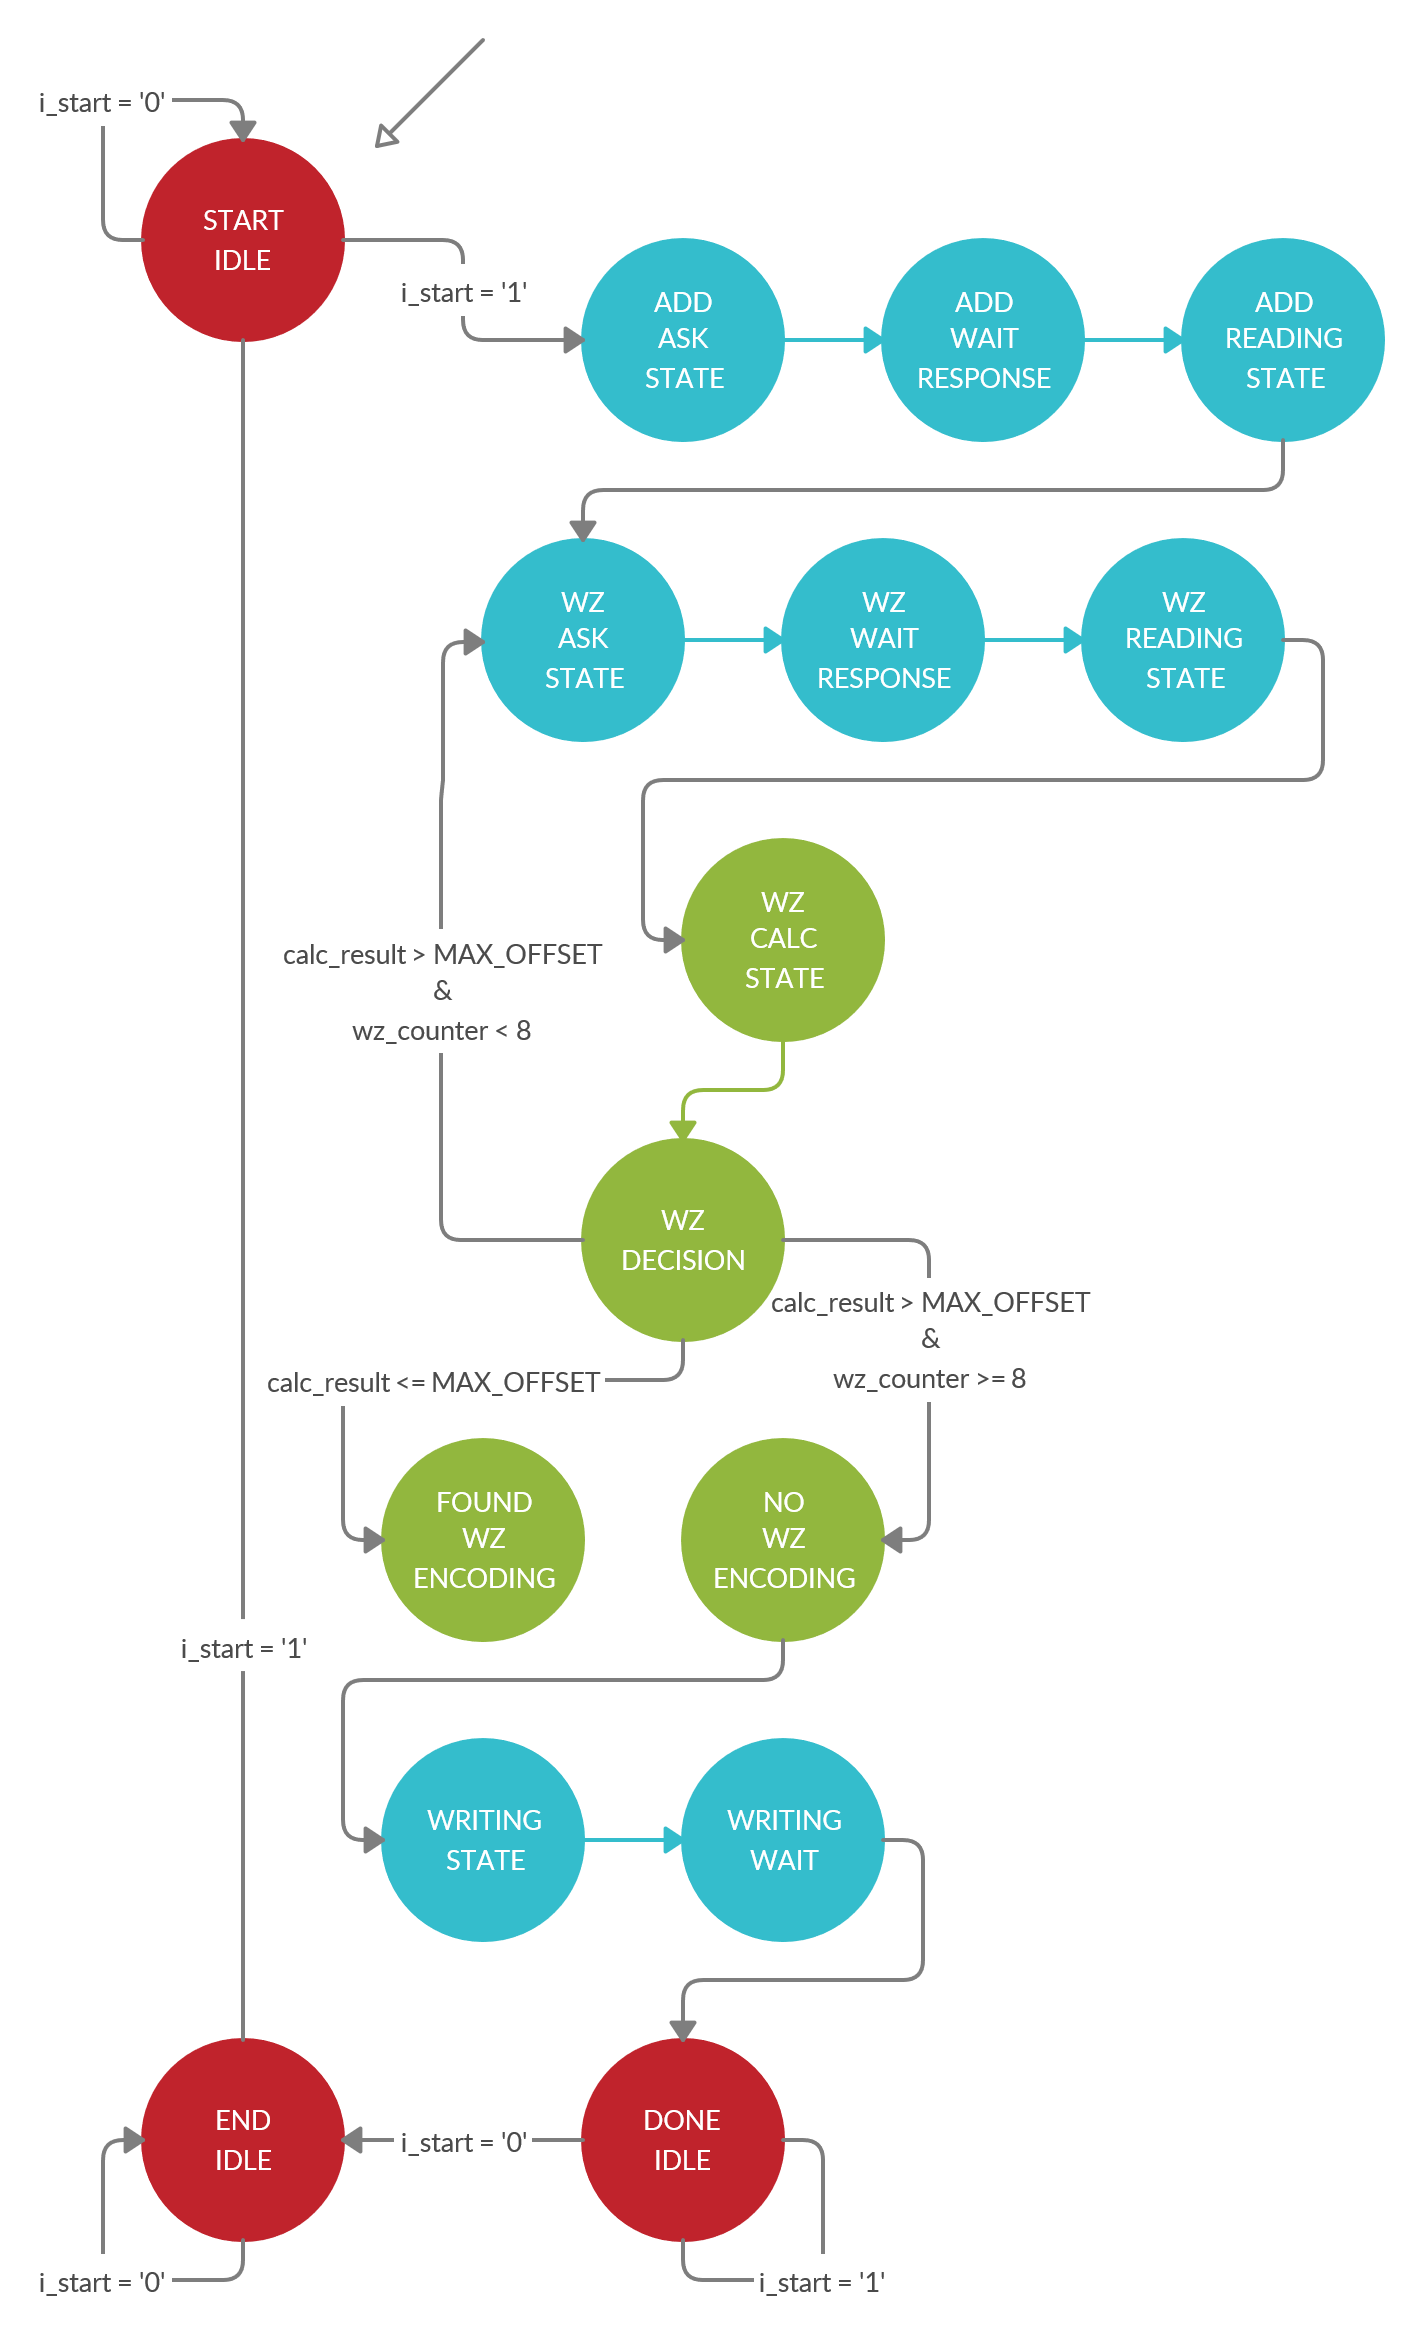
\includegraphics[scale=0.275]{retlog_FSM_v1_2.png}

	\section{Test Eseguiti}
       
		Lorem ipsum dolor sit amet, consectetuer adipiscing elit.  
		Etiam lobortis facilisissem.  Nullam nec mi et neque pharetra 
		sollicitudin.  Praesent imperdiet mi necante...
	\section{Limitazioni e ottimizzazioni possibili}
		\subsection{Hardcoding}
			Gli unici valori hardcodati sono dovuti al formato di codifica del risultato (work in progress)
		\subsection{Segnale di reset}
			Incidentalmente, la macchina viene già inizializzata allo stato di \textit{\texttt{START\_IDLE}}, stato nel quale avviene il reset di tutti i segnali interni e dal quale esce solo tramite il segnale di \textit{\texttt{i\_start}}.
			Ne consegue che \textbf{non è necessario avviare la computazione con il segnale di \textit{\texttt{i\_reset}}}, ma l'utilizzo di \textit{\texttt{i\_reset}} è comunque gestito coerentemente con la specifica. Inoltre, \textit{\texttt{i\_reset}} resetta la macchina riportandone lo stato a \textit{\texttt{START\_IDLE}} indipendentemente dal valore di \textit{\texttt{i\_start}}.
		\subsection{Ottimizzazione dei dati nella RAM}
			La macchina è progettata per produrre il risultato corretto anche se gli indirizzi relativi alle working zone contenuti nella RAM non sono in ordine (vedasi la sezione 3 relativa ai test eseguiti). La macchina infatti esegue una scansione lineare di tutte le working zone, decidendo di volta in volta se richiedere la working zone successiva o fermarsi. Perciò, tra tutte le possibili computazioni il caso pessimo è quello in cui l'indirizzo base non appartiene a nessuna working zone, oppure quello in cui il base address appartiene alla working zone codificata in \textit{\texttt{RAM($7$)}}.
			Tuttavia, se venisse garantito che gli indirizzi delle working zone nella RAM siano in ordine crescente (decrescente), sarebbero possibili due modifiche:
			\begin{itemize}
			\item \textit{Riduzione dei casi pessimi}: se l'indirizzo della working zone appena esaminata ha un valore più alto dell'indirizzo base, si può concludere che l'indirizzo base non appartiene a nessuna working zone, riducendo così il numero dei casi pessimi. Tale modifica al progetto è piuttosto modesta, dal momento che basterebbe modificare lo stato di \textit{\texttt{WZ\_DECISION}}.
			\item \textit{Ricerca binaria}: anziché eseguire una ricerca lineare della working zone risulterebbe più efficiente eseguire una ricerca binaria. Tale strategia ridurrebbe l'intera complessità temporale asintotica della macchina: se $n$ fosse il numero di working zone, si passerebbe da $T(n) \in \mathcal{O}(n)$ a $T(n) \in \mathcal{O}(\log n)$. Tuttavia, questa modifica è più onerosa di quella del punto precedente, dal momento che richiederebbe una modifica all'attuale metodo di scansione (affidato al semplice contatore di working zone \textit{\texttt{wz\_counter}}) e almeno un nuovo stato per il calcolo del prossimo indirizzo di memoria da richiedere.
			\end{itemize}
		\section{Conclusioni}
			Quando non sai che cosa dire, è meglio se non dici nulla
				\newline \newline \newline no scherzo scriviamo che non abbiamo warning
		
\end{document}